\subsubsection{Inner Product Space}

\definecolor{orchid}{HTML}{DA70D6}%
\providecommand{\argmin}{\operatorname*{arg\,min}}%
\providecommand{\argmax}{\operatorname*{arg\,max}}%
\paragraph{Distribution and Test Functions}

\subparagraph{Continous Indexing}

\subparagraph{Duality Pairing}

\subparagraph{Exercises}

\makeatletter
\@ifundefined{mystExerciseSetup}{%
\gdef\mystExerciseSetup{}%
\definecolor{mystExerciseAccent}{HTML}{C2740A}%
\definecolor{mystSolutionAccent}{HTML}{0F766E}%
\newcounter{mystexercise}%
\newenvironment{mystexercise}{%
\par\medskip\refstepcounter{mystexercise}%
\def\FrameCommand{{\color{mystExerciseAccent}\vrule width 3pt}\hspace{10pt}}%
\MakeFramed{\advance\hsize-\width\FrameRestore}%
}{\par\endMakeFramed\medskip}%
\newenvironment{mystsolution}{%
\par\medskip
\def\FrameCommand{{\color{mystSolutionAccent}\vrule width 3pt}\hspace{10pt}}%
\MakeFramed{\advance\hsize-\width\FrameRestore}%
}{\par\endMakeFramed\medskip}%
\newcommand{\mystExHead}[1]{\noindent{\color{mystExerciseAccent}\bfseries Exercise \themystexercise\ (#1)}\par\nobreak\smallskip}%
\newcommand{\mystExHeadPlain}{\noindent{\color{mystExerciseAccent}\bfseries Exercise \themystexercise}\par\nobreak\smallskip}%
\newcommand{\mystSolHead}[1]{\noindent{\color{mystSolutionAccent}\bfseries #1}\par\nobreak\smallskip}%
\newcommand{\mystSolHeadPlain}{\noindent{\color{mystSolutionAccent}\bfseries Solution}\par\nobreak\smallskip}%
}{}%
\makeatother
\begin{mystexercise}\label{delta_as_ring_homomorphism}\mystExHead{$\delta$ is a ring homomorphism}Consider $\mathcal T$ and $\mathbb{R}$ as two rings.

\textbf{1. Prove that $\delta$ preserves ring multiplication}
\begin{equation}
f\delta(x)=f(0)\delta(x)
\end{equation}

\textbf{2. Distribution Derivative of $f\delta$}

Show that the distribution derivative of $f\delta$ is
\begin{equation}
\begin{aligned}
\delta[-fg'] &= f(0)\delta'[g]
\end{aligned}
\end{equation}
or, alternatively,
\begin{equation}
\delta[-fg']= \delta[f'g]+\delta'[fg]
\end{equation}

\end{mystexercise}
\begin{figure}[!htbp]
\centering
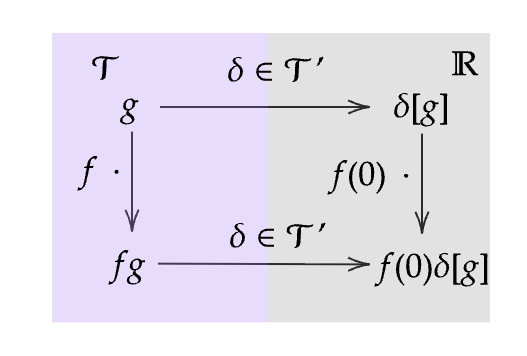
\includegraphics[width=0.7\linewidth]{files/T'_as_module-12b1670b351dbe8ed5bf4d60d4df5809.png}
\end{figure}

\begin{mystsolution}\mystSolHead{Solution to Exercise~\ref{delta_as_ring_homomorphism}}\begin{enumerate}
\item $\forall g\in \mathcal T$, we have:

\begin{equation}
\begin{aligned}
(f\delta)[g] &= \delta[fg] \\
&=f(0)g(0) \\
&= f(0)\delta
\end{aligned}
\end{equation}


As desired.


\item We can direclty compute the derivative:

\begin{equation}
\delta[f\phi] = f(0)\delta[\phi] \overset{\phi=-g'}{\Longrightarrow} \delta[f(-g')] = f(0)\delta[-g'] = f(0)\delta'(g)
\end{equation}


where the last equality used the definition of distribution derivative.
Now we show that $\delta[f'g]+\delta'[fg]=f(0)\delta'(g)$. We use ring homomorphism property to establish:

\begin{equation}
\begin{aligned}
\delta[f'g]+\delta'[fg] &= \delta[f']\delta[g]+\delta[-(fg')] \\
&= \delta[f']\delta[g]-(\delta[f']\delta[g]+\delta[f]\delta[g']) \\
&= -\underbrace{\delta[f]}_{f(0)}\delta[g'] \\
&= f(0)\delta'[g] \\
\end{aligned}
\end{equation}
\end{enumerate}

\end{mystsolution}
\begin{mystexercise}\label{delta_1over2}\mystExHead{$\delta^{(1/2)}$}We can define the distribution $\delta^{(1/2)}$  as a fourier transform of $|k|^{1/2}$:
\begin{equation}
\delta^{(1/2)}=\frac{1}{2\pi}\int_{-\infty}^{\infty} |k|^{1/2}\exp(ikx)dk
\end{equation}

The fourier transform is clearly divergent, hence we can add a regulator. Define:
\begin{equation}
\begin{aligned}
\delta^{(1/2)}_{\mu}&=\frac{1}{2\pi}\int_{-\infty}^{\infty} |k|^{1/2}\exp(ikx)\exp(-\mu|k|)dk \\
&= \frac{1}{2\pi}\int_{-\infty}^{\infty} |k|^{1/2}\exp(ikx-\mu|k|)dk
\end{aligned}
\end{equation}

\begin{enumerate}
\item Evaluate the integral get a closed form expression of $\delta_{\mu}^{(1/2)}$ by:

\begin{itemize}
\item Splitting $k<0$ and $k>0$
\item Change variable to $y=|k|^{1/2}$
\item Write the result as $\frac{d}{d\mu}$ of a Gaussian integral
\item Use the trignometric relation

\begin{equation}
\arctan(z)=\frac{i}{2}\log\left(\frac{1-iz}{1+iz}\right)
\end{equation}
\end{itemize}


\item Investigate $\delta^{(1/2)}_{\mu}$ by:

\begin{itemize}
\item Sketch $\delta^{(1/2)}_{\mu}$ for different $\mu$
\item Compute the zeros of $\delta^{(1/2)}_{\mu}$
\end{itemize}


\item Show that $\delta^{(1/2)}_{\mu}$ is the fourier transform of a function that vanishes at $k=0$. What property of $\delta^{(1/2)}_{\mu}$ can we infer?
\item Compute the limit
$\lim_{\mu \to 0^+}\delta^{(1/2)}_{\mu}$
\item Assuming that for $|x|>\max|\{x_0: \delta^{(1/2)}_{\mu}(x_0)=0\}|$, the convergence of

\begin{equation}
\delta^{(1/2)}_{\mu} \rightarrow \delta^{(1/2)}
\end{equation}


is pointwise. Deduce:

\begin{equation}
\int_{-\infty}^{\infty}\delta^{(1/2)}=-\sqrt{\frac{1}{8\pi}} \int_{-\infty}^{\infty} \frac{1}{|x|^{3/2}}\{\phi(x)-\phi(0)\}dx
\end{equation}
\end{enumerate}

\end{mystexercise}
\begin{mystsolution}\mystSolHead{Solution to Exercise~\ref{delta_1over2}}\begin{enumerate}
\item Following the guide:

\begin{equation}
\begin{aligned}
\delta^{(1/2)}_{\mu} &= \frac{1}{2\pi}\left\{\int_{-\infty}^0 (-k)^{1/2} \exp(ikx+\mu k)dk + \int_{0}^{\infty} (k)^{1/2} \exp(ikx-\mu k)dk 
\right\} \\
&= 
\frac{1}{2\pi}\left\{\underbrace{\int_{-\infty}^0 y \exp(-iy^2x-\mu y^2)dk}_{A} + \underbrace{\int_{0}^{\infty} y\exp(iy^2x-\mu y^2)dk}_{B} 
\right\} \\
\end{aligned}
\end{equation}
\end{enumerate}

\end{mystsolution}
\paragraph{Formal adjoint}

\paragraph{Concrete Adjoint}

\subparagraph{The Sturm-Liouville Operator}

The \textbf{Sturm-Liouville operator} is a linear differential operator of the form
\begin{equation}
\mathcal L=-\frac{d}{dx}\left(p\frac{d}{dx}y\right)+q\frac{d}{dx}
\end{equation}

We've shown that the Sturm-Liouville opeartor is self-adjoint with appropriate boundary condition in the sense that:
\begin{equation}
\begin{aligned}
\langle u, \mathcal Lv \rangle &= \langle \mathcal L^*u, v \rangle
\end{aligned}
\end{equation}
hence it is analgous to self-adjoint operator in finite-dimensional vector spaces, which as symmetric matrix representation when the underlying field is real. We now make this connection explicit, i.e., actually constructing the discretized, finite-dimensional matrix representation of the Sturm-Liouville Operator.

\subparagraph{A Discrete Analog}

Let's consider a concrete SL opeartor defined on $[0,1]$ with Dirchlet boundary condition $y(0)=y(1)=0$. Instead of directly discretizing $\mathcal L$, we aim to find a matrix $L$ such that discretizes the quadratic form:
\begin{equation}
F(y)=\int y\mathcal Ly dx \rightarrow \hat y^TL\hat y
\end{equation}
First we note that:
\begin{equation}
\label{func}
\begin{aligned}
F(y) &= \int_0^1 y\left(-\frac{d}{dx}\left(p\frac{d}{dx}y\right) + qy\right) dx \\
&= \int_0^1 -y \frac{d}{dx}\left(p\frac{d}{dx}y\right)dx+\int_0^1 qy^2dx  \\
&= -\left\{\left[yp\frac{dy}{dx}\right]_0^1 - \int p\left(\frac{dy}{dx}\right)^2 \right\} + \int_0^1 qy^2dx \\
&= \int_0^1 py'^2 + qy^2
\end{aligned}
\end{equation}
Now we discretize $y, p, q$ to $N$-dimensional arrays:
\begin{equation}
\begin{aligned}
\hat y &= [y_1,...,y_N] \\
\hat p &= [p_1,...,p_N] \\
\hat q &= [q_1,...,q_N]
\end{aligned}
\end{equation}
Using forward difference we get:
\begin{equation}
\hat y =\left(\frac{y_{i+1}-y_i}{h}\right)^2
\end{equation}
Rewrite the integral as a finite sum we obtain a discretized version of (\ref{func}):
\begin{equation}
\boxed{\hat F(\hat y)=\sum_{i=1}^N h p_i\left(\frac{y_{i+1}-y_i}{h}\right)^2 +q_iy_i^2}
\end{equation}
Our goal is now to find a matrix $L$ such that $\hat y^TL\hat y=\hat F(\hat y)$. Rewrite $\hat F(\hat y)$:
\begin{equation}
\hat F(\hat y) =\sum_{i=1}^N Np_i(y_{i+1}^2 -2y_{i+1}y_i +y_i^2)+\frac{1}{N}q_iy_i^2
\end{equation}
We can split $L=L_1+L_2$ such that

\begin{enumerate}
\item $\hat y^T L_1 \hat y = \sum_{i=1}^N Np_i(y_{i+1}^2 -2y_{i+1}y_i +y_i^2)$
\item $\hat y^T L_2 \hat y = \sum_{i=1}^N \frac{1}{N}q_iy_i^2$.
\end{enumerate}

\textbf{(Constructing $L_1$)}
Let's first deal with $L_1$. Consider the $2\times 2$block with the upperleft corner at $(i,i)$ that should
represent $Np_i(y_{i+1}^2 -2y_{i+1}y_i +y_i^2)$. This is easy:
\begin{equation}
\begin{aligned}
A_i=Np_i\begin{pmatrix}
1 & -1\\
-1 & 1 \\
\end{pmatrix}
\end{aligned}
\end{equation}
To assemble $L_1$ we can overlap $A_i$ along the diagonal of $L$ with a stride of 1. Concretely:

\begin{verbatim}
for i=1,...,N -1
    L[i,i] += Np_i
    L[i+1,i+1] += Np_i
    L[i,i+1] -= Np_i 
    L[i+1,i] -= Np_i
\end{verbatim}

\begin{example}A quick example for $N=4$:
\begin{equation}
\begin{aligned}
4\begin{pmatrix}
p_1 & -p_1 & 0 & 0 \\
-p_1 & p_1+p_2 & -p_2 &0 \\
0 & -p_2 & p_2+p_3 & -p_3 \\
0 &  0 & -p_3  & p_3
\end{pmatrix}
\end{aligned}
\end{equation}

\end{example}\textbf{(Constructing $L_2$)}
$L_2$ is purely diagonal and is easier to derive. Since it only has quadratic term $y_i^2$, at each row $i$ we only need to include $y_i$. Hence:
\begin{equation}
\begin{aligned}
L_2 = \frac{1}{N}\begin{pmatrix}q_1 & & \\
& \ddots & \\
& & q_N
\end{pmatrix}
\end{aligned}
\end{equation}

\textbf{(Assembly $L_1+L_2$)}
It is clear that $L$ should look like:

\begin{equation}
\begin{aligned}
L=N\begin{pmatrix}
p_1&  -p_1 & & &  \\
-p_1& p_1+p_2 &  -p_2 & &  \\
&  \ddots  &  \ddots &   \ddots &   \\
&  &-p_{N-1} &p_{N-1}+p_{N} & -p_N  \\
& & &-p_N & p_N \\
\end{pmatrix} 
+ 
\frac{1}{N}\begin{pmatrix}q_1 & & \\
& \ddots & \\
& & q_N
\end{pmatrix}
\end{aligned}
\end{equation}

However, since we are dealing with concrete operators with accompanying domain and boundary condition, we need to encoorperate the Dirchelt boundary condition $y(0)=1, y(1)=0$ into $L$. To do so we need to zero-out the first row and column of $L$. Hence finally we get:

\begin{proposition}The Sturm-Liouville Operator on $[0,1]$ with Dirchlet boundary condition $y(0)=y(1)$ can be discretized as
\begin{equation}
\label{discreteSL}
\begin{aligned}
L=N\begin{pmatrix}
0 &0 & & &  &\\
0 &p_1+p_2 & -p_2& & & \\
&-p_2&  \ddots &\ddots & -p_{N-1}& \\
& & \ddots &-p_{N-1} & p_{N-1}+p_N &0 \\
& & & &0 & 0\\
\end{pmatrix} 
+ 
\frac{1}{N}\begin{pmatrix}0 & & & & \\
& q_2 & & & \\
&  & \ddots& & \\
& & & q_{N-1} & \\
& &  & & 0  \\
\end{pmatrix}
\end{aligned}
\end{equation}

\end{proposition}We can see that $L$ is indeed a symmetric real matrix(Hermitian)!

\textbf{Numpy Implementation}
This can easily be translated to naive \texttt{numpy} code:

\begin{verbatim}
class SturmLiouville:
    def __init__(self,N, p, q=None, grid='forward'):
        A = np.zeros(shape=(N,N))
        if grid == 'forward':
            for i in range(N -1):
                A[i, i] += p[i]
                A[i+1, i+1] += p[i]
                A[i, i+1] -= p[i]
                A[i+1, i] -= p[i]

        if q is not None:
            I = np.eye(N) 
            L = A + q @ I
        else:
            L = A
        
        # Dirchlet Boundary Condition
            L[0,0]=0.0
            L[0,1]=0.0
            L[1,0]=0.0
            L[N -1,N -1]=0.0
            L[N -1,N -2]=0.0
            L[N -2,N -1]=0.0
        self.L = (L * N ** 2)
        self.N = N

    def solve_eigen(self, top_k=10):
        eval, evec = np.linalg.eig(self.L)
        top_k_idx = np.argsort(eval[eval>0])[:top_k]
        return eval[top_k_idx] , evec[:, top_k_idx], top_k_idx
\end{verbatim}

\textbf{Example: $-\frac{d^2}{dx^2}$ as a Matrix}
We can do a quick example to showcase that $L$ is indeed a discretization of $\mathcal L$.

\begin{example}[-]\textbf{$\frac{d^2}{dx^2}$}\\
We have already seen that the opeartor:
\begin{equation}
T=-\frac{d^2}{dx^2}, D(T)=\{y,Ty \in L^2[0,1]:y(0)=y(1)=0\}
\end{equation}
has eigenvalues and eigenvectors:
\begin{equation}
\begin{aligned}
y_j(x) &=\sqrt{2}\sin j\pi x \\
\lambda_j &= j^2\pi^2
\end{aligned}
\end{equation}
for $j=1,2,3...$. The problem is that, can we solve a matrix eigenvalue problem to recover exactly the same result?
Indeed we can! Passing $p= -1$ and $q=0$ gets us:
\begin{equation}
\begin{aligned}
L=N\begin{pmatrix}
0 & 0 & &  &  \\
0 & 2 & -1 & &  \\
 & -1 & \ddots & \ddots & \\
& & \ddots & 2 & -1  &\\
& & & -1& 2 & 0\\
& & & & 0 & 0 \\
\end{pmatrix}
\end{aligned}
\end{equation}

and solving the matrix eigenvalue problem
\begin{equation}
\begin{aligned}
L\hat y &= \lambda \hat y
\end{aligned}
\end{equation}
 gets us:
\footnote{Since iterative eigensolvers gives eigenvectors of arbitrary magnitude $v_j=a\sin(j\pi(x))$, we need to normalize properly by
1.Ensure $a>0$

\begin{enumerate}
\item Divide by $\sqrt{\sum y_i^2 h}$
\end{enumerate}}

\begin{figure}[!htbp]
\centering
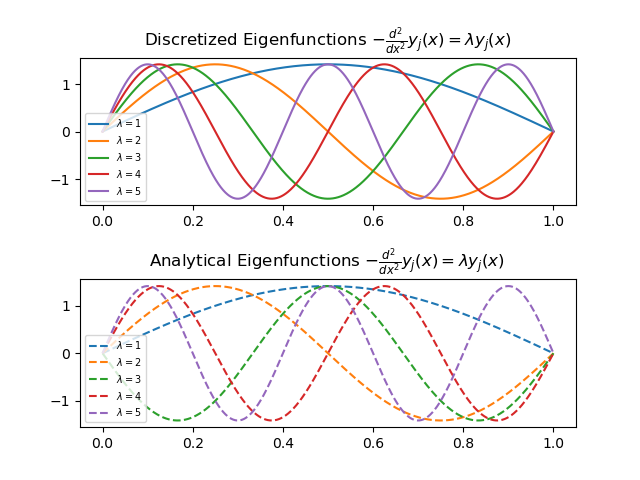
\includegraphics[width=0.7\linewidth]{files/sl_evecs-749bd46b634f4b726002411b1a849030.png}
\end{figure}

\end{example}\begin{mystexercise}\label{exercise-WwKKcCSytY}\label{exercise-wwkkccsyty}\mystExHeadPlain{}\begin{enumerate}
\item We discretized $L$ based on the quadratic form $\int_0^1 y\mathcal L y dx$, hence $\hat y^T L\hat y$ should coincide with $\int_0^1 y\mathcal L y dx$. Come up with at least 2 functions and 2 operators that satisfy the requirment($L^2(0,1),y(0)=y(1)=0$). Compute the quadratic form analytically and numericaly. Cheeck that the results are the same.
\item Remove the masking code snippet(which implements Dirchlet boundary condition) in the naive SL class \texttt{SturmLiouville}. What is the resulting eigenvectors? Explain the result.
\item Try coming up with different discretization with center difference or back difference. Implemet it in \texttt{python}
or \texttt{julia}.

\begin{itemize}
\item Is the resulting matrix $L$ still symmetric ?
\item Center differencing scheme results in a numerical artifcat, what is the numerical artifact? Try explaining why such artifact occur(\textit{Hint: Note that even and oddd indicies are decoupled})
\end{itemize}
\end{enumerate}

\end{mystexercise}
%  
% :::{note} Optimizing $x^TAx$ gives $Ax=\lambda x$
% Let $x\in \mathbb{R}^n$, $A\in \mathbb{R^{n\times n}}$ is a **symmetric** matrix, define:
% $$
% F(x)=\frac12 \langle x,Ax \rangle
% $$
% Consider the optimization of $F$ constrained on $\|x\|^2=1$ 
% :::
% 
% We use lagarange multiplier:
% $$
% (Ax)^T+x^TA-2\lambda x^T &=0 \\
% Ax + A^Tx - 2\lambda x &=0 \\
% 2(A-\lambda I)x&=0 \\
% Ax &= \lambda x
% $$ 
% [^diff]
% Subjected to $\|x\|^2=1$. We note that this is an **eigenvalue problem**. 
%